\chapter{Az alkalmazás funkcionalitásai}

\section{Videólejátszó alapfunkciók}
A alábbi fejezetben az elkészült alkalmazás főbb funkcióit mutatom be, fejtem ki részletesen, külön kitérve a fontosabb, érdekesebb részekre.

A szoftver alapját, magját adó komponens a \textit{VLC} java-n alapuló keretrendszer segítségével valósult meg. Első lépésként a \textit{VLC} videólejátszó megfelelő operációs rendszerre való feltelepítése szükséges. Windows esetén lehet 32 illetve 64 bites verzió. E lépést kötelező megtenni, mivel az fejlesztett alkalmazás a \textit{VLC} lejátszó funkcióit veszi igénybe, nélküle a szoftver nem működik. Ezután a vlcj nevű open source projektet vettem igénybe. Ez Java könyvtárakat ad a \textit{VLC} média lejátszóhoz, így annak majdnem az összes natív funkciója elérhetővé válik a \textit{LibVLC}-n keresztül. Ezen kívül egy keretrendszer használatát is elérhetővé teszi, amely egy egyszerű, magas szintű programozási modellt biztosít, ami magába foglalja a natív könyvtárakhoz való hozzáférést. E keretrendszer amennyire csak lehetséges megvédi a felhasználóját az eredeti könyvár helytelen használatától, ami akár a fejlesztett alkalmazás összeomlását is okozhatja. Segítségével a fejlesztés magas szinten történhetett. Az alkalmazás elindítása után egy egyszerű videó lejátszó kezelőfelülete tárul elénk, amely a \ref{fig:main_screen} ábrán látható.
  
\begin{figure}
\centering
  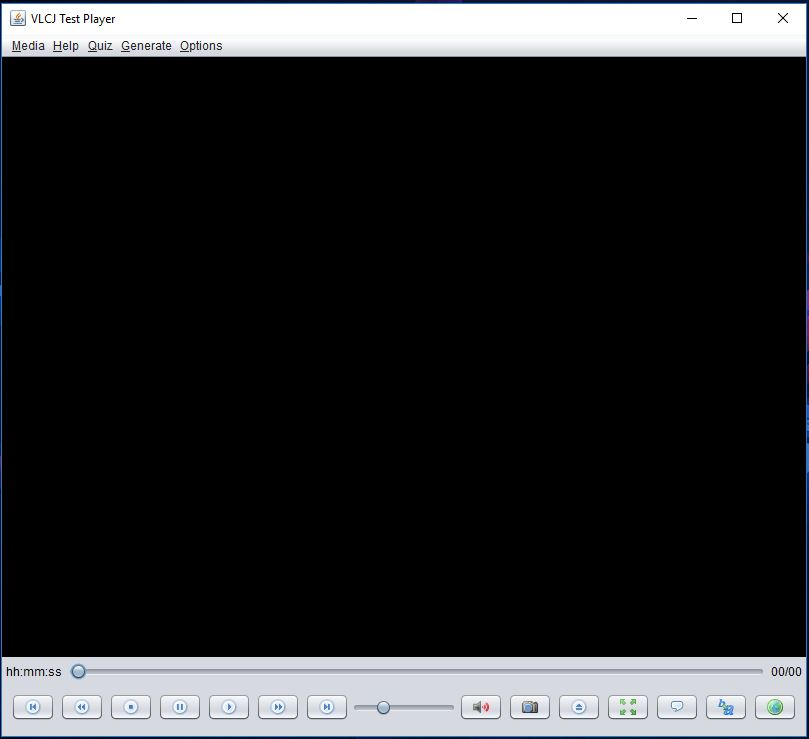
\includegraphics[width=.8\linewidth]{images/main_screen.jpg}
  \caption{Az alkalmazás kezelőfelülete}
  \label{fig:main_screen}
\end{figure}

A képernyő bal alsó sarkában találhatóak meg a videó lejátszását szabályozó gombok. Ezek rendre az előző fejezet, visszatekerés, megállítás, pillanatmegállítás, indítás, előre tekerés, valamint következő fejezet. Középen egy csúszka kapott helyet, amely a hangerőszabályzást teszi lehetővé. Ettől jobbra találhatóak a némító, képernyőfelvétel, médiaválasztó, teljes képernyő, felirat választó, fordítás nyelve, illetve az online feliratok gombok. Ezek működéséről későbbi fejezetekben írok részletesen. Feljebb helyezkedik el a keresősáv, és egy számláló balra, valamint egy jobbra. A bal számláló a lejátszott videó aktuális időpillanatát jelzi, másodperces pontossággal. A csúszka segítségével egyszerűen, intuitívan tekerhetünk a videóban. A jobboldali számláló az aktuális fejezetet mutatja. Az alkalmazás felső részén a menüsáv található, rajta öt különböző menüponttal. Az első segítségével médiafájlokat tallózhatunk, illetve kiléphetünk a szoftverből. A második lehetőség egy segítség opció, a harmadik az ellenőrző kvíz kitöltését teszi lehetővé. A \textit{generate} menüt kibontva PDF fájlt generálhatunk az általunk ismeretlennek vélt szavakból. Felül az utolsó lehetőség a beállítások menüpont, ahol a felirat méretét, illetve késleltetését állíthatjuk be milliszekundumos pontossággal. Ezek áttekintése után már tudunk média fájlokat hozzáadni a szoftverhez. Ehhez kattintsunk az \textit{Eject} gombra az alsó panelről, vagy válasszuk a \textit{Media}, \textit{Play File…} menüpontot. Ekkor megnyílik a felhasználó előtt egy tallózó ablak, ahol böngészhetünk a saját fájlrendszerünkben. Alap beállítás szerint csak a média fájlok jelennek meg az ablakban, azonban ez bármikor felülírható. Itt lehetőség van keresésre, részletes, vagy listás megjelenítésre, feljebb navigálásra, főoldalra való visszatérésre A szoftver képes rengeteg különböző kódolású videó-, és hangfájl lejátszására. Kilépésre a \textit{Cancel} gomb megnyomásával van lehetőség. Ha megtaláltuk a nekünk megfelelő fájlt, a \textit{Play} gombra való kattintással kezdhetjük el a lejátszást. Az ablakot bármikor átméretezhetjük, amivel a benne lejátszott tartalom is méretet vált, fekete sávokkal kitöltve a képaránynak nem megfelelő részeket. Lehetőségünk van a lejátszó némítására, a \textit{Toggle Mute} gombra való kattintással. Ezzel egy időben a gomb ikonja is a megfelelő állapotba vált, jelezve ezzel, hogy a lejátszás le van-e némítva, vagy sem. Az ezt megvalósító kódrészlet \ref{lst:mute}.
\begin{lstlisting}[caption=Némítást implementáló kódrészlet, language=java, label={lst:mute}]
toggleMuteButton.addActionListener(new ActionListener() {
    @Override
    public void actionPerformed(ActionEvent e) {
        mediaPlayer.mute();
        if(mediaPlayer.isMute()){
            toggleMuteButton.setIcon(new ImageIcon(getClass()
            .getClassLoader()
            .getResource("icons/sound.png")));
        } else {
            toggleMuteButton.setIcon(new ImageIcon(getClass()
            .getClassLoader()
            .getResource("icons/sound_mute.png")));
        }
    }
});
\end{lstlisting}

